\chapter{The S4 object system}

R has three object oriented (OO) systems: {[}{[}S3{]}{]}, {[}{[}S4{]}{]}
and {[}{[}R5{]}{]}. This page describes S4.

Compared to S3, the S4 object system is much stricter, and much closer
to other OO systems. I recommend you familiarise yourself with the way
that {[}{[}S3{]}{]} works before reading this document - many of
underlying ideas are the same, but the implementation is much stricter.
There are two major differences from S3:

\begin{itemize}
\item
  formal class definitions: unlike S3, S4 formally defines the
  representation and inheritance for each class
\item
  multiple dispatch: the generic function can be dispatched to a method
  based on the class of any number of argument, not just one
\end{itemize}

Here we introduce the basics of S4, trying to stay away from the
esoterica and focussing on the ideas that you need to understand and
write the majority of S4 code.

\section{Classes and instances}

In S3, you can turn any object into an object of a particular class just
by setting the class attribute. S4 is much stricter: you must define the
representation of the call using \texttt{setClass}, and the only way to
create it is through the constructer function \texttt{new}.

A class has three key properties:

\begin{itemize}
\item
  a \textbf{name}: an alpha-numeric string that identifies the class
\item
  \textbf{representation}: a list of \textbf{slots} (or attributes),
  giving their names and classes. For example, a person class might be
  represented by a character name and a numeric age, as follows:
  \texttt{representation(name = "character", age = "numeric")}
\item
  a character vector of classes that it inherits from, or in S4
  terminology, \textbf{contains}. Note that S4 supports multiple
  inheritance, but this should be used with extreme caution as it makes
  method lookup extremely complicated.
\end{itemize}

You create a class with \texttt{setClass}:

\begin{verbatim}
setClass("Person", representation(name = "character", age = "numeric"))
setClass("Employee", representation(boss = "Person"), contains = "Person")
\end{verbatim}

and create an instance of a class with \texttt{new}:

\begin{verbatim}
hadley <- new("Person", name = "Hadley", age = 31)
\end{verbatim}

Unlike S3, S4 checks that all of the slots have the correct type:

\begin{verbatim}
hadley <- new("Person", name = "Hadley", age = "thirty")
# invalid class "Person" object: invalid object for slot "age" in class
#  "Person": got class "character", should be or extend class "numeric"

hadley <- new("Person", name = "Hadley", sex = "male")
# invalid names for slots of class "Person": sex
\end{verbatim}

If you omit a slot, it will initiate it with the default object of the
class.

To access slots of an S4 object you use \texttt{@}, not \texttt{\$}:

\begin{verbatim}
hadley <- new("Person", name = "Hadley")
hadley@age
# numeric(0)
\end{verbatim}

Or if you have a character string giving a slot name, you use the
\texttt{slot} function:

\begin{verbatim}
slot(hadley, "age")
\end{verbatim}

This is the equivalent of \texttt{{[}{[}}.

An empty value for \texttt{age} is probably not what you want, so you
can also assign a default \textbf{prototype} for the class:

\begin{verbatim}
setClass("Person", representation(name = "character", age = "numeric"), 
  prototype(name = NA_character_, age = NA_real_))
hadley <- new("Person", name = "Hadley")
hadley@age
# [1] NA
\end{verbatim}

\texttt{getSlots} will return a description of all the slots of a class:

\begin{verbatim}
getSlots("Person")
#        name         age 
# "character"   "numeric" 
\end{verbatim}

You can find out the class of an object with \texttt{is}.

Note that there's some tension between the usual interactive functional
style of R and the global side-effect causing S4 class definitions. In
most programming languages, class definition occurs at compile-time,
while object instantiation occurs at run-time - it's unusual to be able
to create new classes interactively. In particular, note that the
examples rely on the fact that multiple calls to \texttt{setClass} with
the same class name will silently override the previous definition
unless the first definition is sealed with \texttt{sealed = TRUE}.

\subsection{Checking validity}

You can also provide an optional method that applies additional
restrictions. This function should have a single argument called
\texttt{object} and should return \texttt{TRUE} if the object is valid,
and if not it should return a character vector giving all reasons it is
not valid.

\begin{verbatim}
check_person <- function(object) {
  errors <- character()
  length_age <- length(object@age)
  if (length_age != 1) {
    msg <- paste("Age is length ", length_age, ".  Should be 1", sep = "")
    errors <- c(errors, msg)
  }

  length_name <- length(object@name)
  if (length_name != 1) {
    msg <- paste("Name is length ", length_name, ".  Should be 1", sep = "")
    errors <- c(errors, msg)
  }
  
  if (length(errors) == 0) TRUE else errors
}
setClass("Person", representation(name = "character", age = "numeric"), 
  validity = check_person)

new("Person", name = "Hadley")
# invalid class "Person" object: Age is length 0.  Should be 1
new("Person", name = "Hadley", age = 1:10)
Error in validObject(.Object) : 
  invalid class "Person" object: Age is length 10.  Should be 1
  
# But note that the check is not automatically applied when we modify 
# slots directly
hadley <- new("Person", name = "Hadley", age = 31)
hadley@age <- 1:10

# Can force check with validObject:
validObject(hadley)
# invalid class "Person" object: Age is length 10.  Should be 1
\end{verbatim}

\section{Generic functions and methods}

Generic functions and methods work similarly to S3, but dispatch is
based on the class of all arguments, and there is a special syntax for
creating both generic functions and new methods.

The \texttt{setGeneric} function provides two main ways to create a new
generic. You can either convert an existing function to a generic
function, or you can create a new one from scratch.

\begin{verbatim}
sides <- function(object) 0
setGeneric("sides")
\end{verbatim}

If you create your own, the second argument to \texttt{setGeneric}
should be a function that defines all the arguments that you want to
dispatch on and contains a call to \texttt{standardGeneric}:

\begin{verbatim}
setGeneric("sides", function(object) {
  standardGeneric("sides")
})
\end{verbatim}

The following example sets up a simple hierarchy of shapes to use with
the sides function.

\begin{verbatim}
setClass("Shape")
setClass("Polygon", representation(sides = "integer"), contains = "Shape")
setClass("Triangle", contains = "Polygon")
setClass("Square", contains = "Polygon")
setClass("Circle", contains = "Shape")
\end{verbatim}

Defining a method for polygons is straightforward: we just use the sides
slot. The \texttt{setMethod} function takes three arguments: the name of
the generic function, the signature to match for this method and a
function to compute the result. Unfortunately R doesn't offer any
syntactic sugar for this task so the code is a little verbose and
repetitive.

\begin{verbatim}
setMethod("sides", signature(object = "Polygon"), function(object) {
  object@sides
})
\end{verbatim}

For the others we supply exact values. Note that that for generics with
few arguments you can simplify the signature without giving the argument
names. This saves spaces at the expense of having to remember which
position corresponds to which argument - not a problem if there's only
one argument.

\begin{verbatim}
setMethod("sides", signature("Triangle"), function(object) 3)
setMethod("sides", signature("Square"),   function(object) 4)
setMethod("sides", signature("Circle"),   function(object) Inf)
\end{verbatim}

You can optionally also specify \texttt{valueClass} to define the
expected output of the generic. This will raise a run-time error if a
method returns output of the wrong class.

\begin{verbatim}
setGeneric("sides", valueClass = "numeric", function(object) {
  standardGeneric("sides")
})
setMethod("sides", signature("Triangle"), function(object) "three")
sides(new("Triangle"))
# invalid value from generic function "sides", class "character", expected
# "numeric"
\end{verbatim}

Note that arguments that the generic dispatches on can't be lazily
evaluated - otherwise how would R know which class the object was? This
also means that you can't use \texttt{substitute} to access the
unevaluated expression.

To find what methods are already defined for a generic function, use
\texttt{showMethods}:

\begin{verbatim}
showMethods("sides")
# Function: sides (package .GlobalEnv)
# object="Circle"
# object="Polygon"
# object="Square"
# object="Triangle"

showMethods(class = "Polygon")
# Function: initialize (package methods)
# .Object="Polygon"
#    (inherited from: .Object="ANY")
# 
# Function: sides (package .GlobalEnv)
# object="Polygon"
\end{verbatim}

\subsection{Method dispatch}

This section describes the strategy for matching a call to a generic
function to the correct method. If there's an exact match between the
class of the objects in the call, and the signature of a method, it's
easy - the generic function just calls that method. Otherwise, R will
figure out the method using the following method:

\begin{itemize}
\item
  For each argument to the function, calculate the distance between the
  class in the class, and the class in the signature. If they are the
  same, the distance is zero. If the class in the signature is a parent
  of the class in the call, then the distance is 1. If it's a
  grandparent, 2, and so on. Compute the total distance by adding
  together the individual distances.
\item
  Calculate this distance for every method. If there's a method with a
  unique smallest distance, use that. Otherwise, give a warning and call
  one of the matching methods as described below.
\end{itemize}

Note that it's possible to create methods that are ambiguous - i.e.~it's
not clear which method the generic should pick. In this case R will pick
the method that is first alphabetically and return a warning message
about the situation:

\begin{verbatim}
setClass("A")
setClass("A1", contains = "A")
setClass("A2", contains = "A1")
setClass("A3", contains = "A2")

setGeneric("foo", function(a, b) standardGeneric("foo")) 
setMethod("foo", signature("A1", "A2"), function(a, b) "1-2")
setMethod("foo", signature("A2", "A1"), function(a, b) "2-1")

foo(new("A2"), new("A2"))
# Note: Method with signature "A2#A1" chosen for function "foo",
# target signature "A2#A2". "A1#A2" would also be valid
\end{verbatim}

Generally, you should avoid this ambiguity by providing a more specific
method:

\begin{verbatim}
setMethod("foo", signature("A2", "A2"), function(a, b) "2-2")
foo(new("A2"), new("A2"))
\end{verbatim}

(The computation is cached for this combination of classes so that it
doesn't have to be done again.)

There are two special classes that can be used in the signature:
\texttt{missing} and \texttt{ANY}. \texttt{missing} matches the case
where the argument is not supplied, and \texttt{ANY} is used for setting
up default methods. \texttt{ANY} has the lowest possible precedence in
method matching.

You can also use basic classes like \texttt{numeric}, \texttt{character}
and \texttt{matrix}. A matrix of (e.g.) characters will have class
\texttt{matrix}.

\begin{verbatim}
setGeneric("type", function(x) standardGeneric("type"))
setMethod("type", signature("matrix"), function(x) "matrix")
setMethod("type", signature("character"), function(x) "character")

type(letters)
type(matrix(letters, ncol = 2))
\end{verbatim}

You can also dispatch on S3 classes provided that you have made S4 aware
of them by calling \texttt{setOldClass}.

\begin{verbatim}
foo <- structure(list(x = 1), class = "foo")
type(foo)

setOldClass("foo")
setMethod("type", signature("foo"), function(x) "foo")

type(foo)

setMethod("+", signature(e1 = "foo", e2 = "numeric"), function(e1, e2) {
  structure(list(x = e1$x + e2), class = "foo")
})
foo + 3
\end{verbatim}

It's also possible to dispatch on \texttt{...} under special
circumstances. See \texttt{?dotsMethods} for more details.

\subsection{Inheritance}

Let's develop a fuller example. This is inspired by an example from the
\href{http://www.opendylan.org/gdref/tutorial.html}{Dylan language
reference}, one of the languages that inspired the S4 object system. In
this example we'll develop a simple model of vehicle inspections that
vary depending on the type of vehicle (car or truck) and type of
inspector (normal or state).

In S4, it's the \texttt{callNextMethod} that (surprise!) is used to call
the next method. It figures out which method to call by pretending the
current method doesn't exist, and looking for the next closest match.

First we set up the classes: two types of vehicle (car and truck), and
two types of inspect.

\begin{verbatim}
setClass("Vehicle")
setClass("Truck", contains = "Vehicle")
setClass("Car", contains = "Vehicle")

setClass("Inspector", representation(name = "character"))
setClass("StateInspector", contains = "Inspector")
\end{verbatim}

Next we define the generic function for inspecting a vehicle. It has two
arguments: the vehicle being inspected and the person doing the
inspection.

\begin{verbatim}
setGeneric("inspect.vehicle", function(v, i) {
   standardGeneric("inspect.vehicle")
 })
\end{verbatim}

All vehicle must be checked for rust by all inspectors, so we'll add the
first. Cars also need to have working seatbelts.

\begin{verbatim}
setMethod("inspect.vehicle", 
 signature(v = "Vehicle", i = "Inspector"), 
 function(v, i) {
   message("Looking for rust")
 })

setMethod("inspect.vehicle", 
 signature(v = "Car", i = "Inspector"),
 function(v, i) {  
   callNextMethod() # perform vehicle inspection
   message("Checking seat belts")
 })

 inspect.vehicle(new("Car"), new("Inspector"))
 # Looking for rust
 # Checking seat belts
\end{verbatim}

Note that it's the most specific method that's responsible for ensuring
that the more generic methods are called.

We'll next add methods for trucks (cargo attachments need to be ok), and
the special task that the state inspected performs on cars: checking for
insurance.

\begin{verbatim}
setMethod("inspect.vehicle", 
  signature(v = "Truck", i = "Inspector"),
  function(v, i) {
    callNextMethod() # perform vehicle inspection
    message("Checking cargo attachments")
  })

inspect.vehicle(new("Truck"), new("Inspector"))
# Looking for rust
# Checking cargo attachments

setMethod("inspect.vehicle", 
  signature(v = "Car", i = "StateInspector"),
  function(v, i) {
    callNextMethod() # perform car inspection
    message("Checking insurance")
})

inspect.vehicle(new("Car"), new("StateInspector"))
# Looking for rust
# Checking seat belts
# Checking insurance
\end{verbatim}

This set up ensures that when a state inspector checks a truck, they
perform all of the checks a regular inspector would:

\begin{verbatim}
 inspect.vehicle(new("Truck"), new("StateInspector"))
 # Looking for rust
 # Checking cargo attachments
\end{verbatim}

\section{Method dispatch 2}

To make the ideas in this section concrete, we'll create a simple class
structure. We have three classes, C which inherits from a character
vector, B inherits from C and A inherits from B. We then instantiate an
object from each class.

\begin{Shaded}
\begin{Highlighting}[]
\KeywordTok{setClass}\NormalTok{(}\StringTok{"C"}\NormalTok{, }\DataTypeTok{contains =} \StringTok{"character"}\NormalTok{)}
\KeywordTok{setClass}\NormalTok{(}\StringTok{"B"}\NormalTok{, }\DataTypeTok{contains =} \StringTok{"C"}\NormalTok{)}
\KeywordTok{setClass}\NormalTok{(}\StringTok{"A"}\NormalTok{, }\DataTypeTok{contains =} \StringTok{"B"}\NormalTok{)}

\NormalTok{a <-}\StringTok{ }\KeywordTok{new}\NormalTok{(}\StringTok{"A"}\NormalTok{, }\StringTok{"a"}\NormalTok{)}
\NormalTok{b <-}\StringTok{ }\KeywordTok{new}\NormalTok{(}\StringTok{"B"}\NormalTok{, }\StringTok{"b"}\NormalTok{)}
\NormalTok{c <-}\StringTok{ }\KeywordTok{new}\NormalTok{(}\StringTok{"C"}\NormalTok{, }\StringTok{"c"}\NormalTok{)}
\end{Highlighting}
\end{Shaded}

This creates a class graph that looks like this:

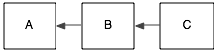
\includegraphics{diagrams/class-graph-1.png}

Next, we create a generic f, which will dispatch on two arguments:
\texttt{x} and \texttt{y}.

\begin{Shaded}
\begin{Highlighting}[]
\KeywordTok{setGeneric}\NormalTok{(}\StringTok{"f"}\NormalTok{, function(x, y) }\KeywordTok{standardGeneric}\NormalTok{(}\StringTok{"f"}\NormalTok{))}
\end{Highlighting}
\end{Shaded}

To predict which method a generic will dispatch to, you need to know:

\begin{itemize}
\itemsep1pt\parskip0pt\parsep0pt
\item
  the name and arguments to the generic
\item
  the signatures of the methods
\item
  the class of arguments supplied to the generic
\end{itemize}

The simplest type of method dispatch occurs if there's an exact match
between the class of arguments (arg-classes) and the signature of
(sig-classes). In the following example, we define methods with
sig-classes \texttt{c("C", "C")} and \texttt{c("A", "A")}, and then call
them with arg classes \texttt{c("C", "C")} and \texttt{c("A", "A")}.

\begin{Shaded}
\begin{Highlighting}[]
\KeywordTok{setMethod}\NormalTok{(}\StringTok{"f"}\NormalTok{, }\KeywordTok{signature}\NormalTok{(}\StringTok{"C"}\NormalTok{, }\StringTok{"C"}\NormalTok{), function(x, y) }\StringTok{"c-c"}\NormalTok{)}
\KeywordTok{setMethod}\NormalTok{(}\StringTok{"f"}\NormalTok{, }\KeywordTok{signature}\NormalTok{(}\StringTok{"A"}\NormalTok{, }\StringTok{"A"}\NormalTok{), function(x, y) }\StringTok{"a-a"}\NormalTok{)}

\KeywordTok{f}\NormalTok{(c, c)}
\KeywordTok{f}\NormalTok{(a, a)}
\end{Highlighting}
\end{Shaded}

If there isn't an exact match, R looks for the closest method. The
distance between the sig-class and arg-class is the sum of the distances
between each class (matched by named and excluding \ldots{}). The
distance between classes is the shortest distance between them in the
class graph. For example, the distance A -\textgreater{} B is 1, A
-\textgreater{} C is 2 and B -\textgreater{} C is 1. The distances C
-\textgreater{} B, C -\textgreater{} A and B -\textgreater{} A are all
infinite. That means that of the following two calls will dispatch to
the same method:

\begin{Shaded}
\begin{Highlighting}[]
\KeywordTok{f}\NormalTok{(b, b)}
\KeywordTok{f}\NormalTok{(a, c)}
\end{Highlighting}
\end{Shaded}

If we added another class, BC, that inherited from both B and C, then
this class would have distance one to both B and C, and distance two to
A. As you can imagine, this can get quite tricky if you have a
complicated class graph: for this reason it's better to avoid multiple
inheritance unless absolutely necessary.

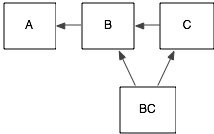
\includegraphics{diagrams/class-graph-2.png}

\begin{Shaded}
\begin{Highlighting}[]
\KeywordTok{setClass}\NormalTok{(}\StringTok{"BC"}\NormalTok{, }\DataTypeTok{contains =} \KeywordTok{c}\NormalTok{(}\StringTok{"B"}\NormalTok{, }\StringTok{"C"}\NormalTok{))}
\NormalTok{bc <-}\StringTok{ }\KeywordTok{new}\NormalTok{(}\StringTok{"BC"}\NormalTok{, }\StringTok{"bc"}\NormalTok{)}
\end{Highlighting}
\end{Shaded}

Let's add a more complicated case:

\begin{verbatim}
setMethod("f", signature("B", "C"), function(x, y) "b-c")
setMethod("f", signature("C", "B"), function(x, y) "c-b")
f(b, b)
\end{verbatim}

Now we have two signatures that have the same distance (1 = 1 + 0 = 0 +
1), and there is not unique closest method. In this situation R gives a
warning and calls the method that comes first alphabetically.

There are two special classes that can be used in the signature:
\texttt{missing} and \texttt{ANY}. \texttt{missing} matches the case
where the argument is not supplied, and \texttt{ANY} is used for setting
up default methods. \texttt{ANY} has the lowest possible precedence in
method matching - in other words, it has a distance value higher than
any other parent class.

\begin{Shaded}
\begin{Highlighting}[]
\KeywordTok{setMethod}\NormalTok{(}\StringTok{"f"}\NormalTok{, }\KeywordTok{signature}\NormalTok{(}\StringTok{"C"}\NormalTok{, }\StringTok{"ANY"}\NormalTok{), function(x,y) }\StringTok{"C-*"}\NormalTok{)}
\KeywordTok{setMethod}\NormalTok{(}\StringTok{"f"}\NormalTok{, }\KeywordTok{signature}\NormalTok{(}\StringTok{"C"}\NormalTok{, }\StringTok{"missing"}\NormalTok{), function(x,y) }\StringTok{"C-?"}\NormalTok{)}

\KeywordTok{setClass}\NormalTok{(}\StringTok{"D"}\NormalTok{, }\DataTypeTok{contains =} \StringTok{"character"}\NormalTok{)}
\NormalTok{d <-}\StringTok{ }\KeywordTok{new}\NormalTok{(}\StringTok{"D"}\NormalTok{, }\StringTok{"d"}\NormalTok{)}

\KeywordTok{f}\NormalTok{(c)}
\KeywordTok{f}\NormalTok{(c, d)}
\end{Highlighting}
\end{Shaded}

It's also possible to dispatch on \texttt{...} under special
circumstances. See \texttt{?dotsMethods} for more details.

\section{In the wild}

To conclude, lets look at some S4 code in practice. The Bioconductor
\texttt{EBImage}, by Oleg Sklyar, Gregoire Pau, Mike Smith and Wolfgang
Huber, package is a good place to start because it's so simple. It has
only one class, an \texttt{Image}, which represents a image as an array
of pixel values.

\begin{verbatim}
setClass ("Image",
  representation (colormode="integer"),
  prototype (colormode=Grayscale),
  contains = "array"
)

imageData = function (y) {
  if (is(y, 'Image')) y@.Data
  else y
}    
\end{verbatim}

The author wrote the \texttt{imageData} convenience method to extract
the underlying S3 object, the array. They could have also used the
\texttt{S3Part} function to extract this.

Methods are used to define numeric operations for combining two images,
or an image with a constant. Here the author is using the \texttt{Ops}
group generic which will match all calls to \texttt{+}, \texttt{-},
\texttt{*}, \texttt{\^{}}, \texttt{\%\%}, \texttt{\%/\%}, \texttt{/},
\texttt{==}, \texttt{\textgreater{}}, \texttt{\textless{}}, \texttt{!=},
\texttt{\textless{}=}, \texttt{\textgreater{}=}, \texttt{\&}, and
\texttt{\textbar{}}. The \texttt{callGeneric} function then passed on
this call to the generic method for arrays. Finally, each method checks
that the modified object is valid, before returning it.

\begin{verbatim}
setMethod("Ops", signature(e1="Image", e2="Image"),
    function(e1, e2) {
          e1@.Data=callGeneric(imageData(e1), imageData(e2))
           validObject(e1)
          return(e1)
    }
)
setMethod("Ops", signature(e1="Image", e2="numeric"),
    function(e1, e2) {
          e1@.Data=callGeneric(imageData(e1), e2)
          validObject(e1)
          return(e1)
    }
)
setMethod("Ops", signature(e1="numeric", e2="Image"),
    function(e1, e2) {
          e2@.Data=callGeneric(e1, imageData(e2))
          validObject(e2)
          return(e2)
    }
)
\end{verbatim}

The \texttt{Matrix} package by Douglas Bates and Martin Maechler is a
great example of a more complicated setup. It is designed to efficiently
store and compute with many different special types of matrix. As at
version 0.999375-50 it defines 130 classes and 24 generic functions. The
package is well written, well commented and fairly easy to read. The
accompanying
\href{http://cran.r-project.org/web/packages/Matrix/vignettes/Intro2Matrix.pdf}{vignette}
gives a good overview of the structure of the package. I'd highly
recommend downloading the source and then skimming the following R
files:

\begin{itemize}
\item
  \texttt{AllClass.R}: where all classes are defined
\item
  \texttt{AllGenerics.R}: where all generics are defined
\item
  \texttt{Ops.R}: where pairwise operators are defined, including
  automatic conversion of standard S3 matrices
\end{itemize}

Most of the hard work is done in C for efficiency, but it's still useful
to look at the other R files to see how the code is arranged.
